%!TEX root = main.tex

\section{How do software developers \textbf{plan} for merge conflict resolutions? (RQ2)}\label{RQ2}

\boldif{Developers use different strategies for dealing with MC}
When encountering a merge conflict, developers follow different strategies.
They can either: (a) defer the merge conflict to a later date, or; (b) solve the conflict.
In the \textit{Processes Survey} we sought an understanding of these strategies and when developers use them.
The tools that developers use when implementing merge conflict resolutions are discussed in Section~\ref{RQ5}.

\subsection{Deferring Responses to Merge Conflicts}

\boldif{25\% of developers consider all conflicts as being equally urgent.}
One quarter of our participants consider all merge conflicts to be equally urgent.
This means that they will always solve the conflict as soon as the 
We can assume that most developers will interrupt their work regardless of the type of merge conflict.
Therefore, they will give the same level of attention, for example, to a conflict generated by whitespace or formatting changes, as a conflict that is generated by overlapping logical changes. 
%TODO: Make sure this fits in the flow.

\boldif{The first option is that they might defer the MC, for a later time}
The easiest option when encountering a merge conflict is to simply not deal with it.
Indeed, we found that 56.18\% of participants have deferred at least once when responding to a merge conflict.
The reasons for deferring are varied and listed in Table~\ref{s1_deferring_response}.

The location and complexity of conflicting code (D1, D2) were the most selected factors, and match the top difficulty factors of merge conflicts (F1, F2) as described in Section~\ref{difficulty-factors}.
% TODO Add a conclusion statement about the meaning of these factors being top in both tables.

As the third most selected factor, \textit{ownership of the conflicting code}~(D3) indicates that the deferral is not always temporal, but can also be logistical when developers defer to other team members.
A \textit{Barriers Survey} participant succinctly defines the role ownership impacts his workflow as:
\begin{quotation}
	Code is mine? I fix it. Code is others? I submit PR or bug reports.
\end{quotation}
We additionally asked participants to rate the degree to which code ownership factors into their overall merge conflict strategy, and participants indicate that code ownership factors \textit{about half the time} in their strategy of code ownership (mean: $3.21$ on a 5-point Likert-type scale).
Only 10.11\% of participants indicated that code ownership \textit{never} factors into their resolution strategy.

\begin{table}[!htbp]
\renewcommand{\arraystretch}{1.2}
\caption{Factors in Deferring Responses to Merge Conflicts from \textit{Processes Survey}}
\label{s1_deferring_response}
\centering
\begin{tabularx}{\textwidth}{c|Q{8.45cm}|cr}
\toprule
  \rowcolor[gray]{0.85}
  \parnoteclear % tabularx will otherwise add each note thrice
  Factor & Description & Selections\parnote{\label{factors}\textit{Processes Survey} participants were allowed to select multiple factors. 44 out of 102 participants (43\%) selected more than one factor.\vspace*{-0.9\baselineskip}} & Percentage\parnoteref{factors} \\
\midrule
  D1 & Complexity of the conflicting code & 36 & (25.00\%) \\
  \rowcolor[gray]{0.95}D2 & Number of conflicting code locations & 32 & (22.22\%) \\
  D3 & Ownership of the conflicting code & 25 & (17.36\%) \\
  \rowcolor[gray]{0.95}D4 & Size of the conflicting code & 20 & (13.89\%) \\
  D5 & Approaching deadlines & 13 & (9.03\%) \\
  \rowcolor[gray]{0.95}D6 & Work schedule constraints & 2 & (1.39\%) \\
  D7 & Other\hspace{4.6cm} & 7 & (4.86\%) \\
\bottomrule
\end{tabularx}
\parnotes
\end{table}

\boldif{60\% of developers defer a merge conflict, at least once. However, there doesn't seem to be a systematic understanding of the effect of such a deferral.}
%Our study results indicate that 60\% of developers have deferred a merge conflict at least once. 
While developers have listed multiple reasons for deferral, two stand out: complexity and the number of conflicting locations.
Both of these reasons indicate that a developer is more likely to defer if the conflict resolution appears to be lengthy, either because the potential changes are non-trivial or because there are many smaller conflicts requiring the developers' attention.

\boldif{Deferring can have bad consequences, including increased complexity and delaying features. Organizations have sometimes changed the policy to prevent this.}
Deferring the merge conflict resolution comes with a price.
Table~\ref{effects-deferral} shows the top effects of deferring a response to a merge conflict.
The most common effect was that developers have had to stop the development (\emph{Stop the Presses,} 15 responses) in order to resolve the conflicts.
This halt in development includes asking team members to also refrain from adding any additional code into the codebase.
The second most common effect is the \textit{increased complexity} of the conflicts (E2), reported by nine participants.
A \textit{Barriers Survey} participant noted that:
\begin{quotation}
	Deferring a merge conflict simply kicks the can down the road (or off a cliff). Typically resolving the conflict only gets more difficult as time passes.
\end{quotation}
Another participant even hinted that the increased complexity can be quite severe, on an order of magnitude greater than if the conflict were addressed immediately:
\begin{quotation}
	Untangling takes days instead of minutes when it gets too out of hand.
\end{quotation}
In some cases, features had to be removed from releases, in order for integration problems to be mitigated and the conflict to be successfully resolved. One participant said:
\begin{quotation}
	We have had several releases come up short in new features because they got delayed by integration problems.
\end{quotation}
In order to prevent similar problems arising, some organizations have instituted \textit{policy changes} (E4) to prevent this from happening in the future.
However, the survey participants that selected \textit{policy changes} (E4) had a mean of 10.2 years of software development experience, which is higher than the overall mean of 9.1 years.
The awareness of policy changes that were introduced specifically to address merge conflicts might be higher among senior developers.
A \textit{Barriers Survey} participant said:
\begin{quotation}
	We've had devs push a bunch of code up before going on holiday and mucking up a release, so we've instituted an all hands on deck policy for the 2 weeks leading up to a major release
\end{quotation}

\boldif{However, some effect can be severe, including impact to customers, or having to reimplement features.}
In one extreme case, a participant reported that an unresolved merge conflict affected production software (E7), which resulted in downtime of the product, as it broke functionality:
\begin{quotation}
	Broke the app for customers until we could get a patch pushed [\ldots].
\end{quotation}
Finally, the merge conflicts can get too severe and intractable for developers to cope with the complexities.
In these types of situations, developers have to resort to the \emph{Nuclear Option} (E5), where they scrap their changes and manually reimplement them.
Such as in the case of one participant, who said:
\begin{quotation}
	Uh.... KABOOM! More changes came in and everything piled up. Nothing to do but wipe it all back to clean and start trying to piece things back together.
\end{quotation}

\begin{table}[!htbp]
\renewcommand{\arraystretch}{1.2}
\caption{Effects of Deferring Response to a Merge Conflict from \textit{Processes Survey}}
\label{effects-deferral}
\centering
\begin{tabularx}{\textwidth}{c|Q{8.18cm}|cr}
\toprule
  \rowcolor[gray]{0.85}
  \parnoteclear % tabularx will otherwise add each note thrice
  Effect & Description & Participants\parnote{\label{effects}46 out of 102 participants (45.1\%) provided a description of the effects of deferring.\vspace*{-0.8\baselineskip}} & Percentage\parnoteref{effects} \\
\midrule
  E1 & Stop the Presses & 15 & (32.61\%) \\
  \rowcolor[gray]{0.95}E2 & Increased complexity & 9 & (19.57\%) \\
  E3 & Non-operation effects & 5 & (10.87\%) \\
  \rowcolor[gray]{0.95}E4 & Policy/cultural changes & 3 & (6.52\%) \\
  E5 & The Nuclear Option & 2 & (4.35\%) \\
  \rowcolor[gray]{0.95}E6 & Physical manifestations & 1 & (2.17\%) \\
  E7 & Impact beyond the organization & 2 & (2.17\%) \\
\bottomrule
\end{tabularx}
\parnotes
\end{table}

\boldif{The results of such a deferral can be disastrous. However, it is difficult to make an assessment of the effect of the deferral when the decision to defer is being made.} 
The results of deferring can be disastrous. 
%Participants reported having to throw away code (the \emph{Nuclear Option}) and even rising to the level of customers and users experiencing broken functionality and loss of access.
However, it is difficult to assess a deferral to determine if it will turn a single merge conflict into a larger problem.
Tools could provide such information; responding to developers with enough information to make accurate and informed decisions in order to prevent further issues down the line.\vspace{1cm}

\subsection{Resolution Attempts \& Strategies}

\boldif{If they have not deferred, they need to understand the (changes in the) conflict}
When developers don't defer their response, they have to resolve the conflicts now.
They primarily approach merge conflicts by \textit{examining the merge} (U1), \textit{analyzing or manipulating the code} (U2), or \textit{examining the code} (U3); where the main difference between examining the merge and examining the code is that code involves developing an understanding of one set of changes.
Understanding a merge conflict, on the other hand, required understanding two sets of change \emph{and their interaction.}
As discussed in Section~\ref{sec:rw:pc}, this imposes a considerably higher cognitive load on the developer.
Table~\ref{s1_understanding_code} lists all six strategies described by the \textit{Processes Survey} participants.

\begin{table}[!htbp]
\renewcommand{\arraystretch}{1.2}
\caption{Initial Strategies for Understanding Conflicting Code from \textit{Processes Survey}}
\label{s1_understanding_code}
\centering
\begin{tabularx}{\textwidth}{c|Q{7.75cm}|cr}
\toprule
  \rowcolor[gray]{0.85}
  \parnoteclear % tabularx will otherwise add each note thrice
  Strategy & Description & Participants\parnote{\label{understanding}79 out of 102 participants (77\%) provided a description of their initial strategy.\vspace*{-0.3\baselineskip}} & Percentage\parnoteref{understanding} \\
\midrule
  U1 & Examining the merge & 26 & (32.91\%) \\
  \rowcolor[gray]{0.95}U2 & Analysis/manipulation of the code & 19 & (24.05\%) \\
  U3 & Examining the code & 18 & (22.79\%) \\
  \rowcolor[gray]{0.95}U4 & Focus on design concerns & 8 & (10.13\%) \\
  U5 & Examine project organization & 6 & (7.60\%) \\
  \rowcolor[gray]{0.95}U6 & No strategy & 2 & (2.53\%) \\
\bottomrule
\end{tabularx}
\parnotes
\end{table}

\boldif{The most common strategies for understanding the conflict are examining the conflict and analysis/manipulation of the code.}
A \textit{Processes Survey} participant described their strategy of \textit{examining the merge}~(U1) as:
\begin{quotation}
	Reviewing the most recent commits (comments and code) to see whether it's a shallow conflict or not.
\end{quotation}
	And another participant indicated their strategy of analyzing the code (U2) involves:
\begin{quotation}
[\ldots] determining if the merge conflict involves important functionality; stepping through with a debugger helps.
\end{quotation}
Overall, we find that developers initially focus on the code involved in the merge conflict or information related to the merge itself.

\boldif{Surprisingly, some developers do not have a strategy for MCR}
Surprisingly, we found that two of our participants (2.53\% of participants) indicated that they \textit{``don't have a strategy''} or \textit{``mostly try to fix it as soon as possible.''}

%\begin{figure}[!htbp]
%\centering
%\fbox{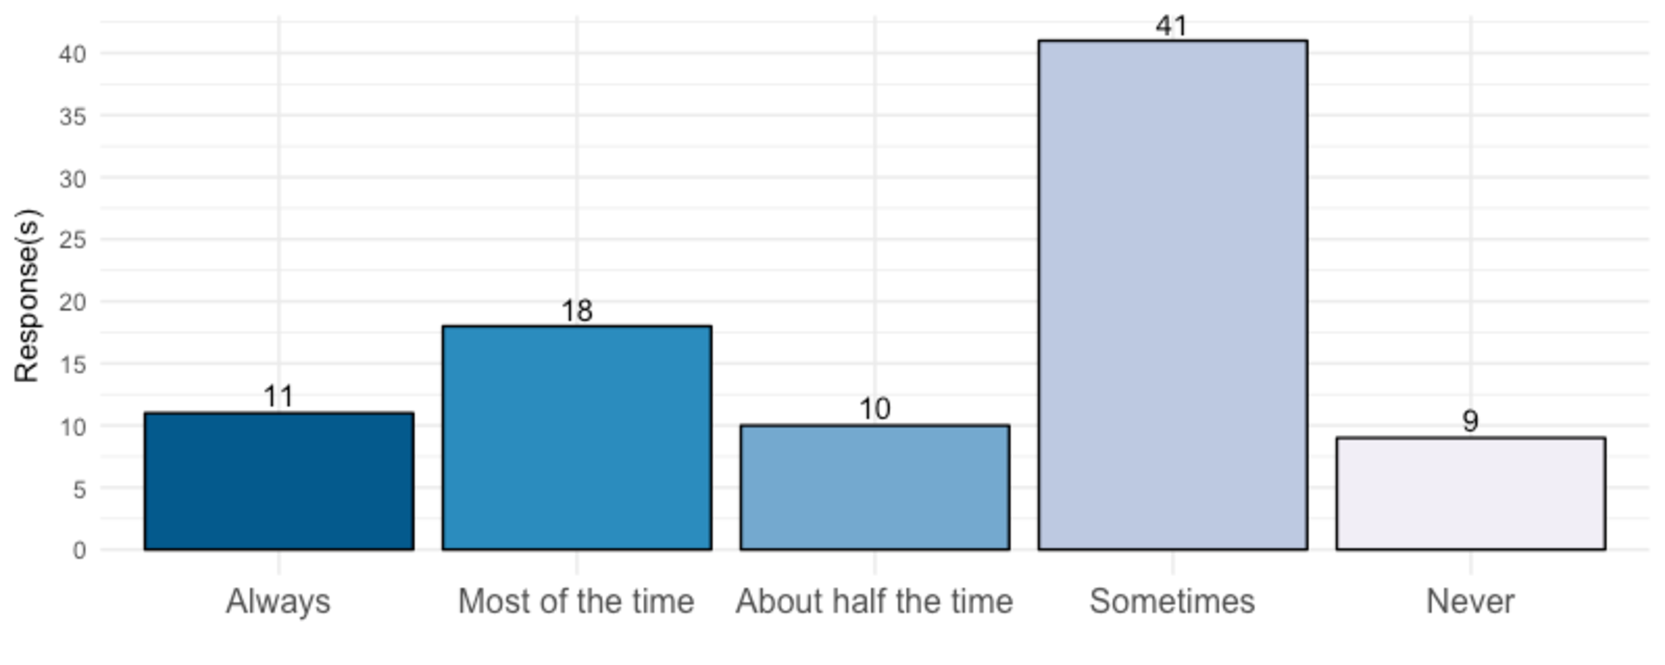
\includegraphics[width=0.98\textwidth,keepaspectratio]{imgs/CodeOwnershipFactor}}
%\caption{Degree of Code Ownership as a Factor in Merge Conflict Strategies. Scale: 1 is \textit{Always} and 5 is \textit{Never}. 89 out of 102 participants (87.26\%) provided a response to this question in the \textit{Processes Survey}.\vspace*{-0.3\baselineskip}}
%\label{fig:code-ownership-resolution}
%\end{figure}

To conclude, developers reported that expertise in the area of the conflicting code is one of the top factors in determining the difficulty of a merge conflict.
Additionally, developers also indicate that increases in perceived complexity of merge conflicts is strongly linked with the degree of difficulty in resolving them.
Therefore, developers' perceptions and intuition are relied on throughout the implementation of their resolution.